% -*- mode: LaTeX; compile-command: "pdflatex CS-history.tex" -*-

\documentclass[xcolor={usenames,dvipsnames,svgnames,table},12pt]{beamer}

\mode<presentation>
{
  \usetheme{default}                          % use a default (plain) theme

  \setbeamertemplate{navigation symbols}{}    % don't show navigation
                                              % buttons along the
                                              % bottom
  \setbeamerfont{normal text}{family=\sffamily}

%  \setbeamertemplate{footline}[frame number]

  \AtBeginSection[]
  {
    \begin{frame}<beamer>
      \frametitle{}
      \begin{center}
        {\Huge \insertsectionhead}

        % \vspace{0.25in}
        % \includegraphics[width=2in]{\secimage}
      \end{center}
    \end{frame}
  }
}

\newenvironment{xframe}[1][]
  {\begin{frame}[fragile,environment=xframe,#1]}
  {\end{frame}}

% uncomment me to get 4 slides per page for printing
% \usepackage{pgfpages}
% \pgfpagesuselayout{4 on 1}[uspaper, border shrink=5mm]

% \setbeameroption{show only notes}

\usepackage[english]{babel}
\usepackage[T1]{fontenc}
\usepackage{graphicx}
\graphicspath{{images/}}

\usepackage{ulem}
\usepackage{url}
\usepackage{fancyvrb}

\title{Computer Science History}
% \date{}
% \author{Dr.\ Brent Yorgey}

%%%%%%%%%%%%%%%%%%%%%%%%%%%%%%%%%%%%%%%%%%%%%%%%%%%%%%%%%%%%%%%%%%%

\begin{document}

% \maketitle

\begin{frame}
  \begin{center}
    When was the first mechanical computer made?
  \end{center}
\end{frame}

\begin{frame}{Antikythera Mechanism}
  \begin{center}
    \raisebox{-0.5\height}{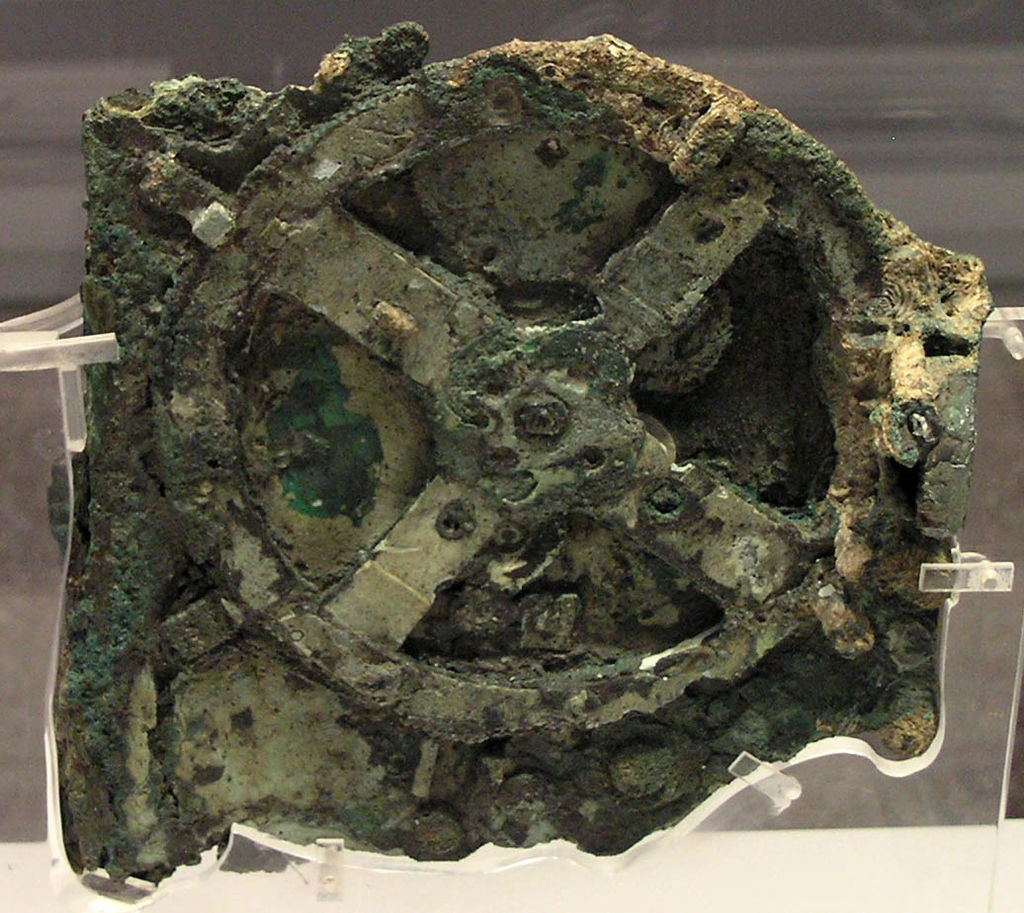
\includegraphics[width=2in]{antikythera1.jpeg}} \quad
    \raisebox{-0.5\height}{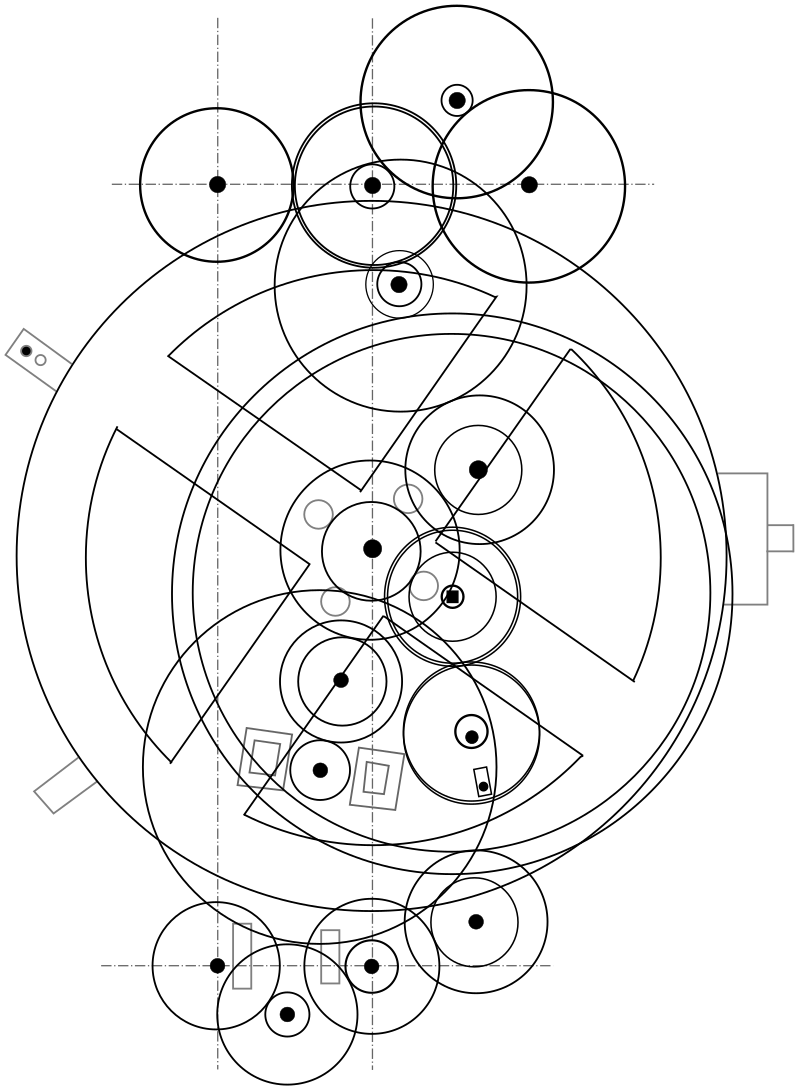
\includegraphics[width=2in]{Antikythera-gears.png}} \\
    100-200 BC?  Discovered 1901
  \end{center}
\end{frame}

\begin{frame}{}
  \begin{center}
    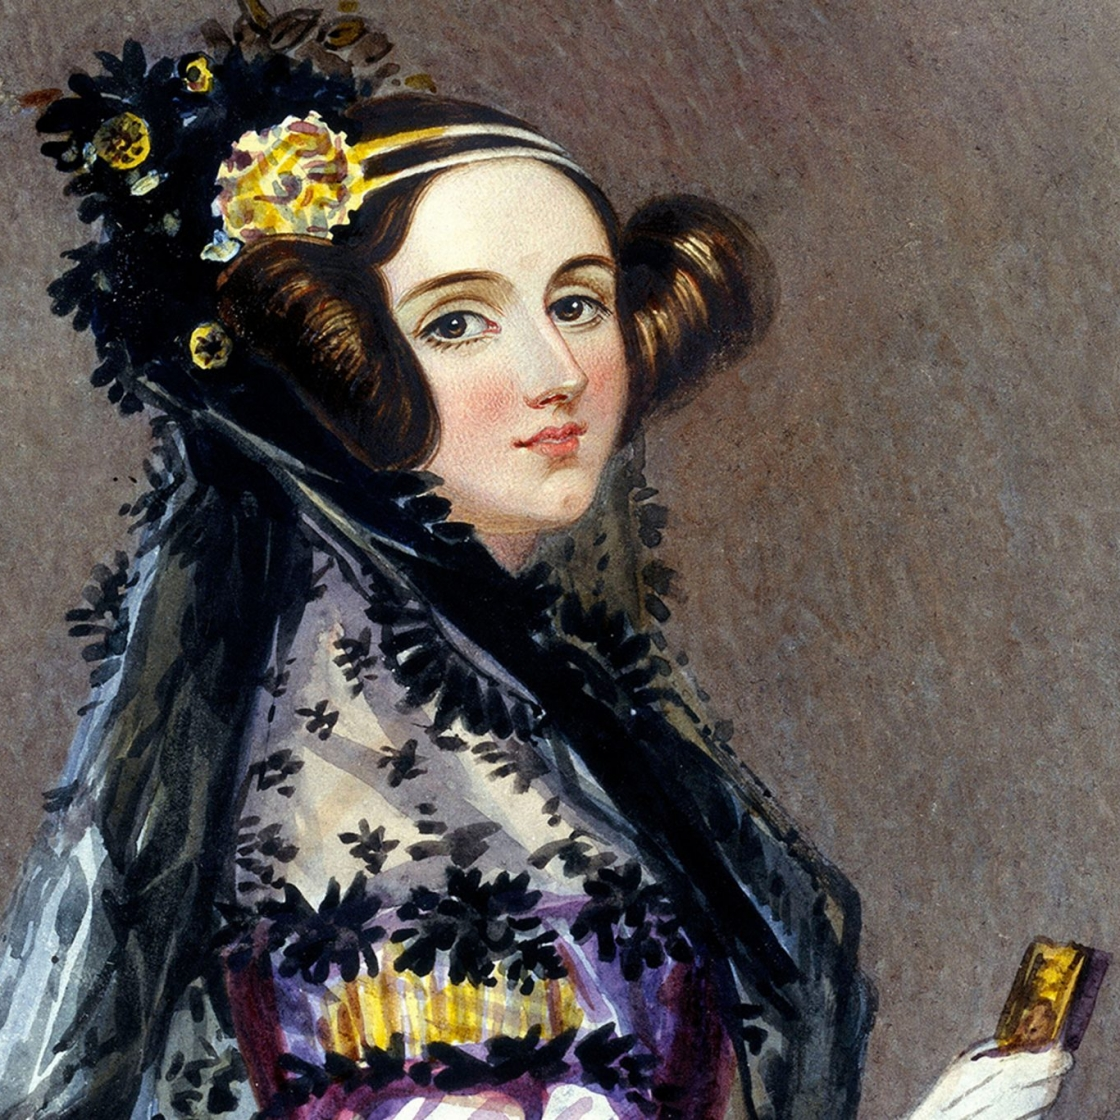
\includegraphics[height=2in]{ada-lovelace}
    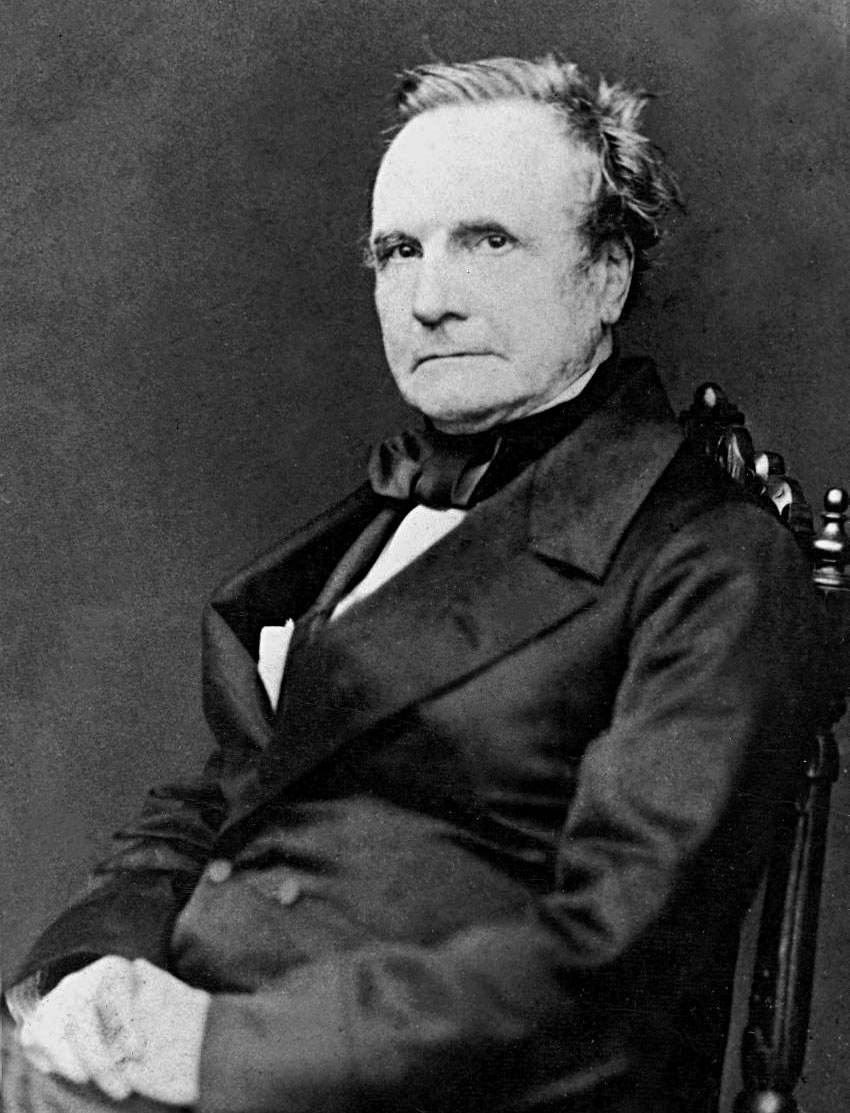
\includegraphics[height=2in]{Babbage}
  \end{center}
\end{frame}

\begin{frame}{Lovelace and Babbage}
  \begin{center}
    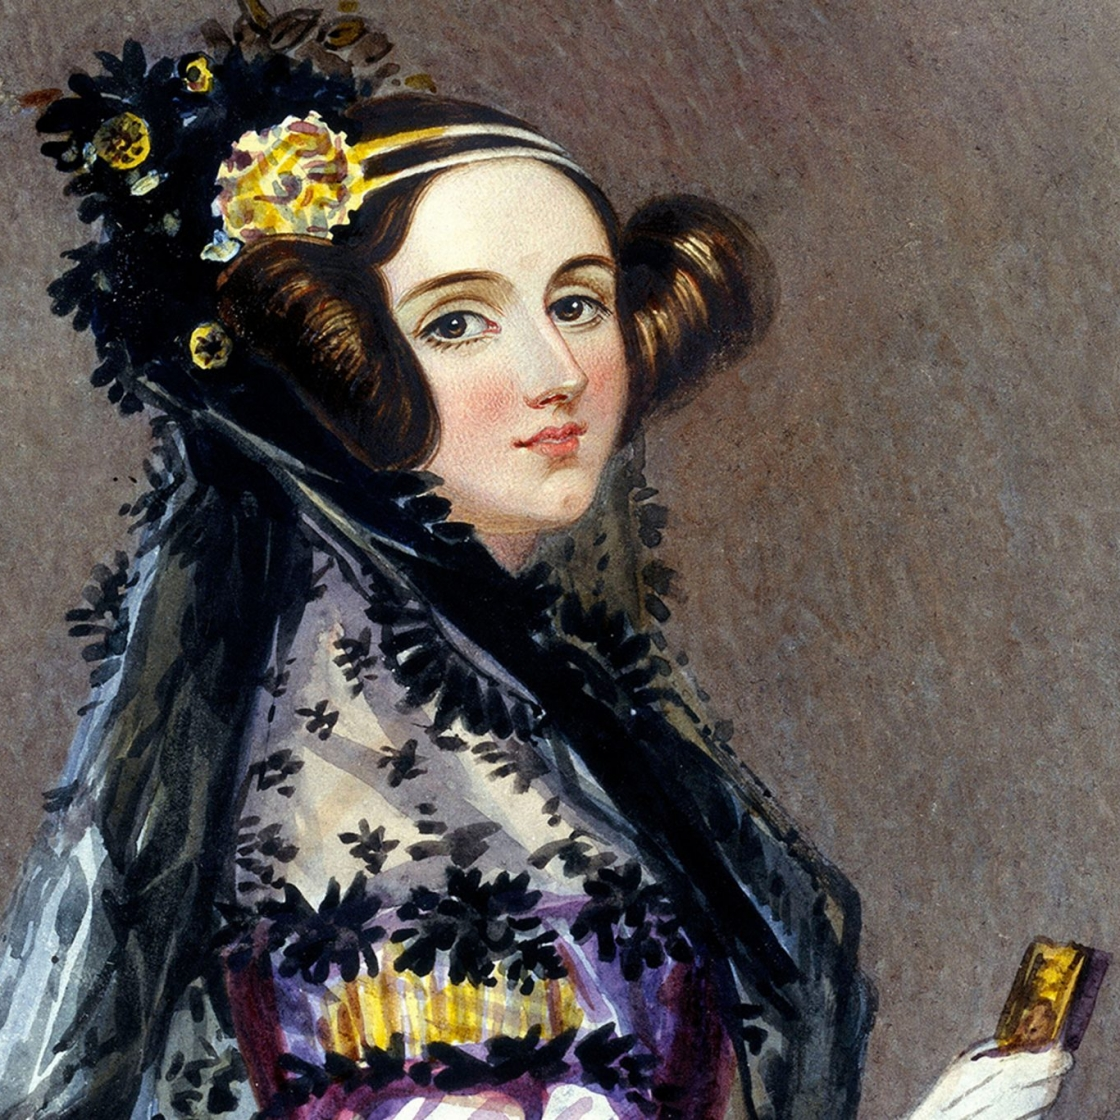
\includegraphics[height=2in]{ada-lovelace}
    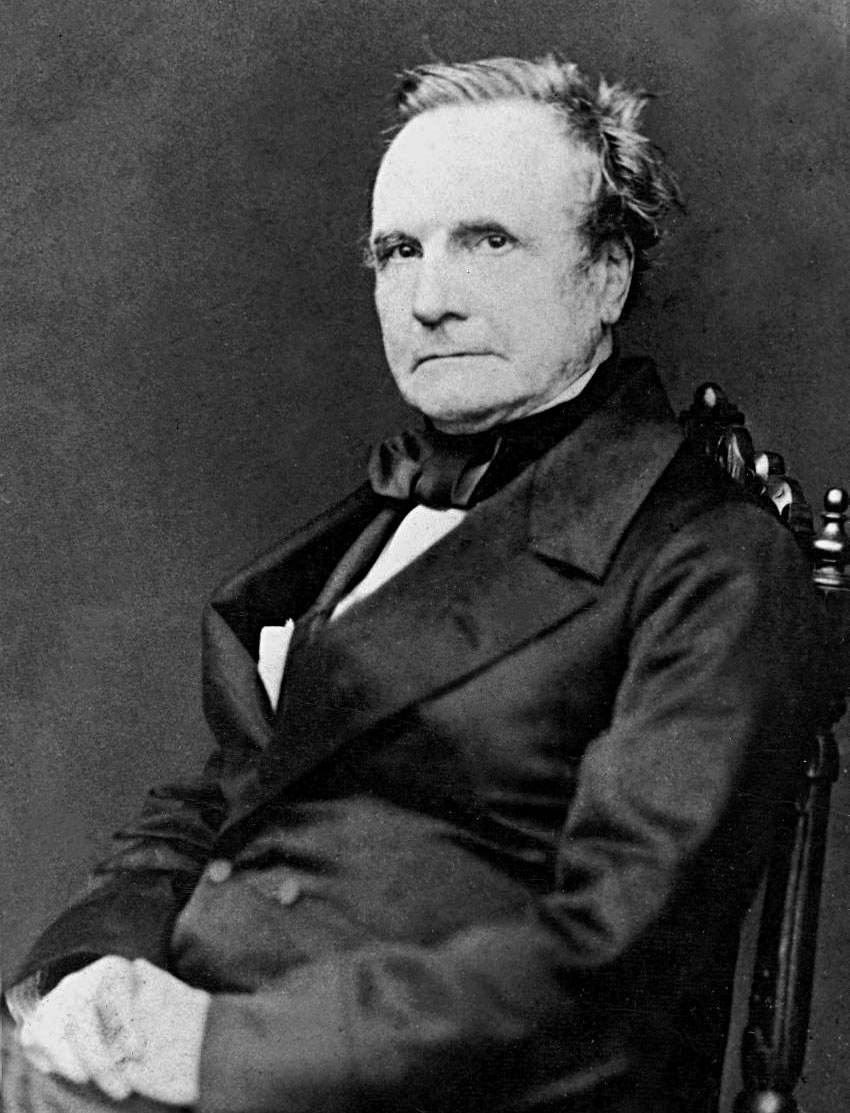
\includegraphics[height=2in]{Babbage}

    Ada Augusta King, Countess of Lovelace (1815--1852)\\
    Charles Babbage (1791--1871)
  \end{center}
\end{frame}

\begin{frame}{The first computer program?}
  \begin{center}
    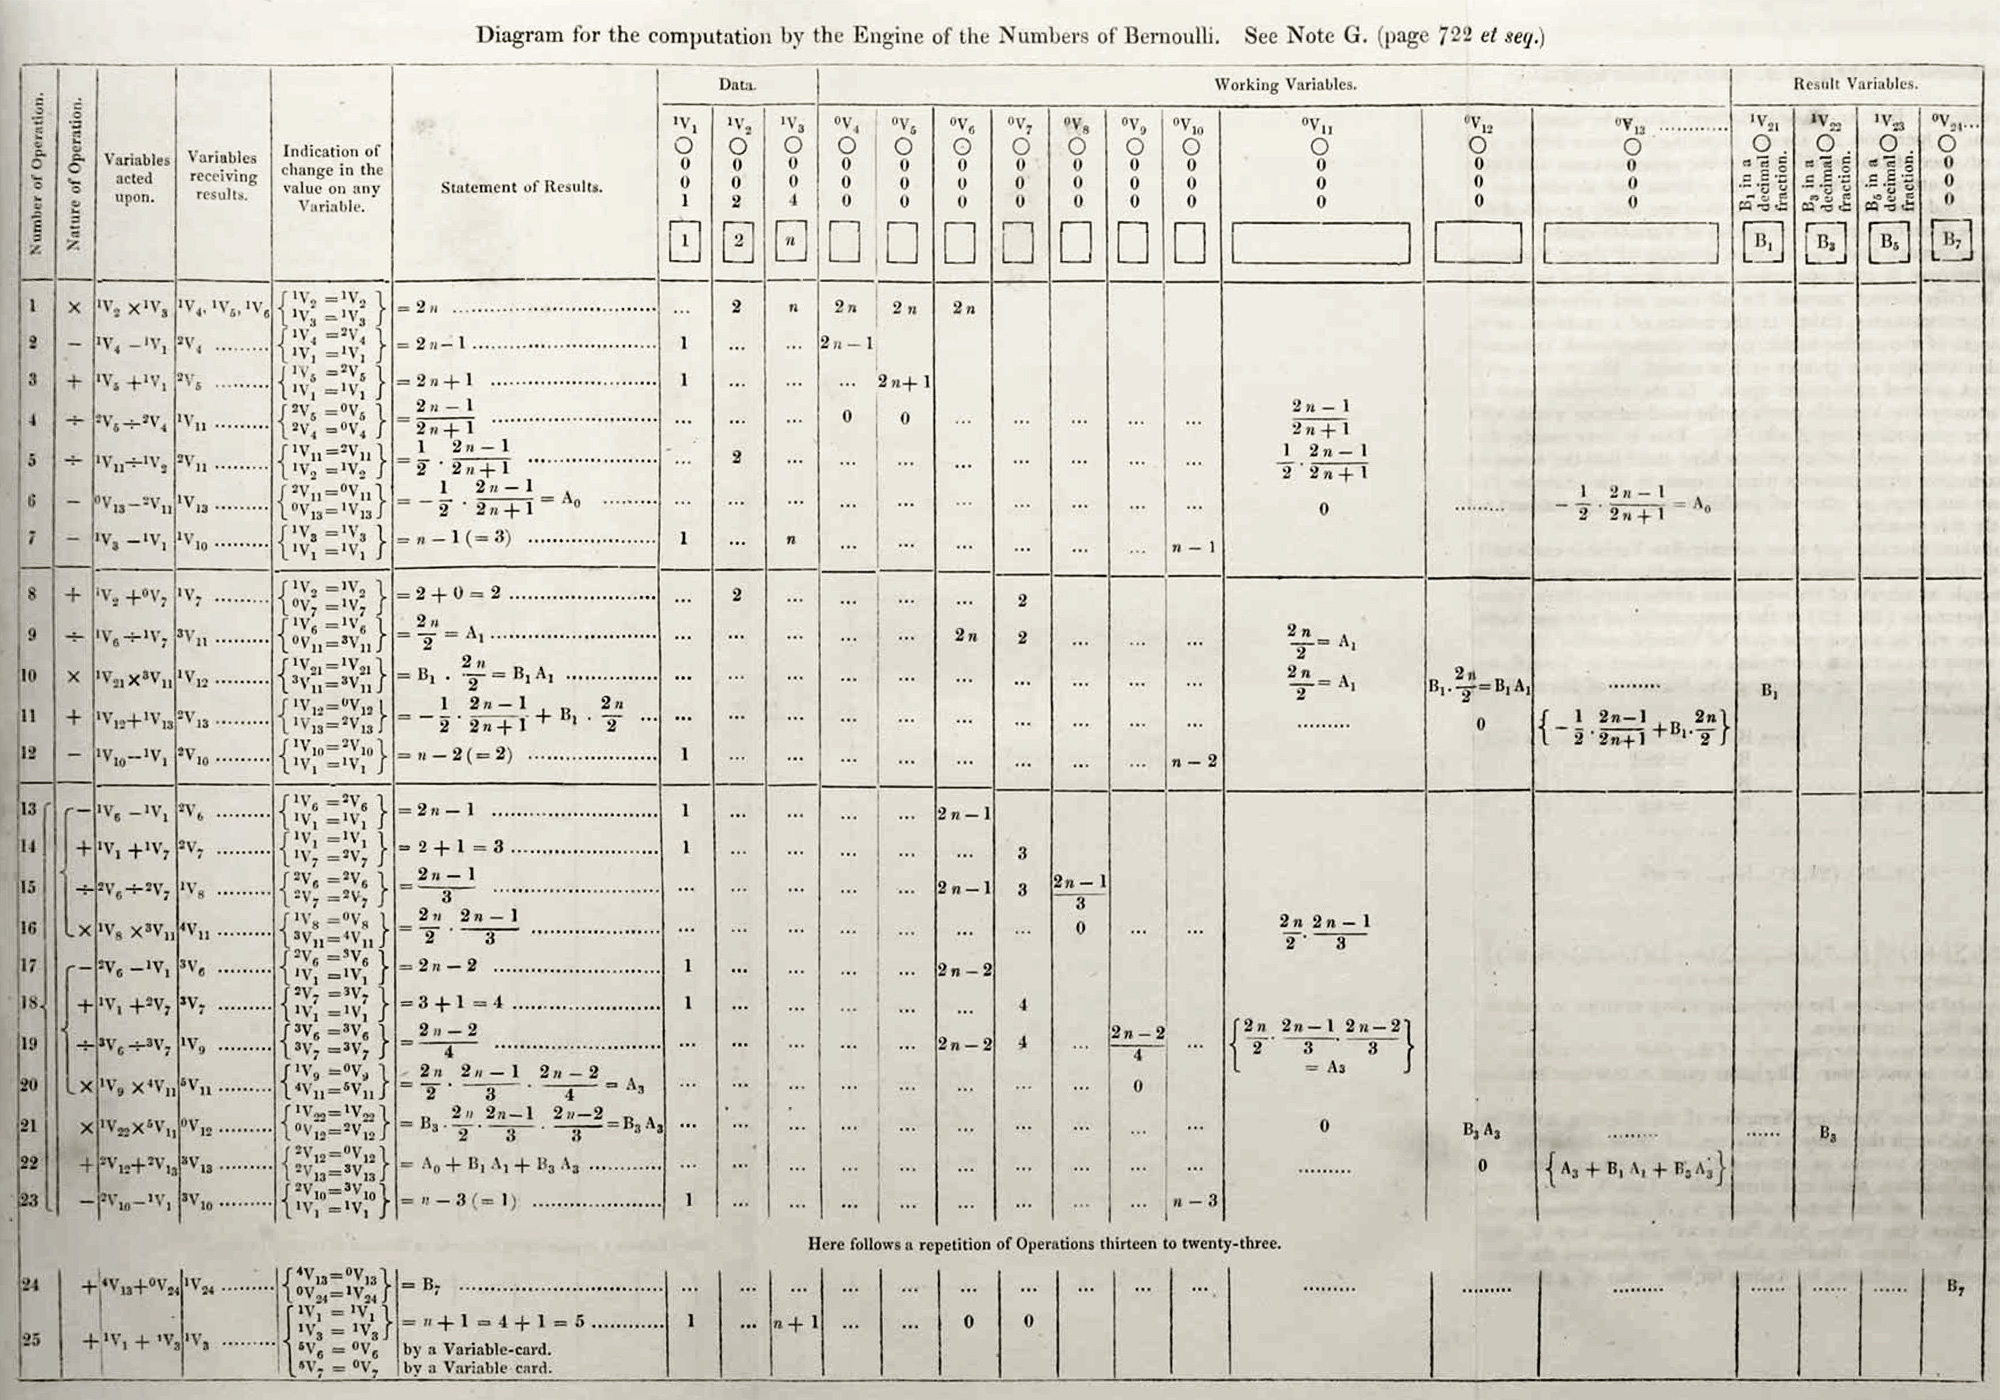
\includegraphics[width=4in]{lovelace-program}
  \end{center}
\end{frame}

% \begin{frame}{}
%   \begin{quote}
%     ``[The Analytical Engine] might act upon other things besides number,
%     were objects found whose mutual fundamental relations could be
%     expressed by those of the abstract science of operations, and which
%     should be also susceptible of adaptations to the action of the
%     operating notation and mechanism of the engine\dots \medskip

%     Supposing, for instance, that the fundamental relations of pitched
%     sounds in the science of harmony and of musical composition were
%     susceptible of such expression and adaptations, the engine might
%     compose elaborate and scientific pieces of music of any degree of
%     complexity or extent.''
%   \end{quote}
% \end{frame}

\begin{frame}{}
  \begin{center}
    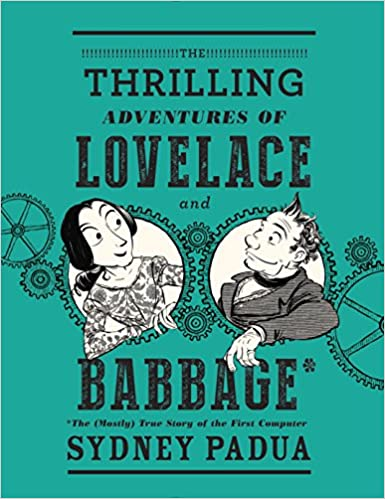
\includegraphics[width=2in]{adventures}
  \end{center}
\end{frame}

\begin{frame}{}
  \begin{center}
    When was the first electronic computer made?
  \end{center}
\end{frame}

\begin{frame}{Colossus}
  \begin{center}
    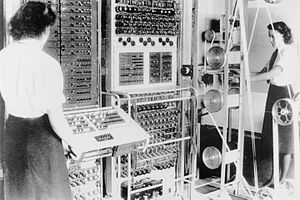
\includegraphics[width=2in]{Colossus}

    1943--45, first programmable, electronic, digital computer \\
    Secret until 1970s!
  \end{center}
\end{frame}

\begin{frame}{ENIAC}
  \begin{center}
    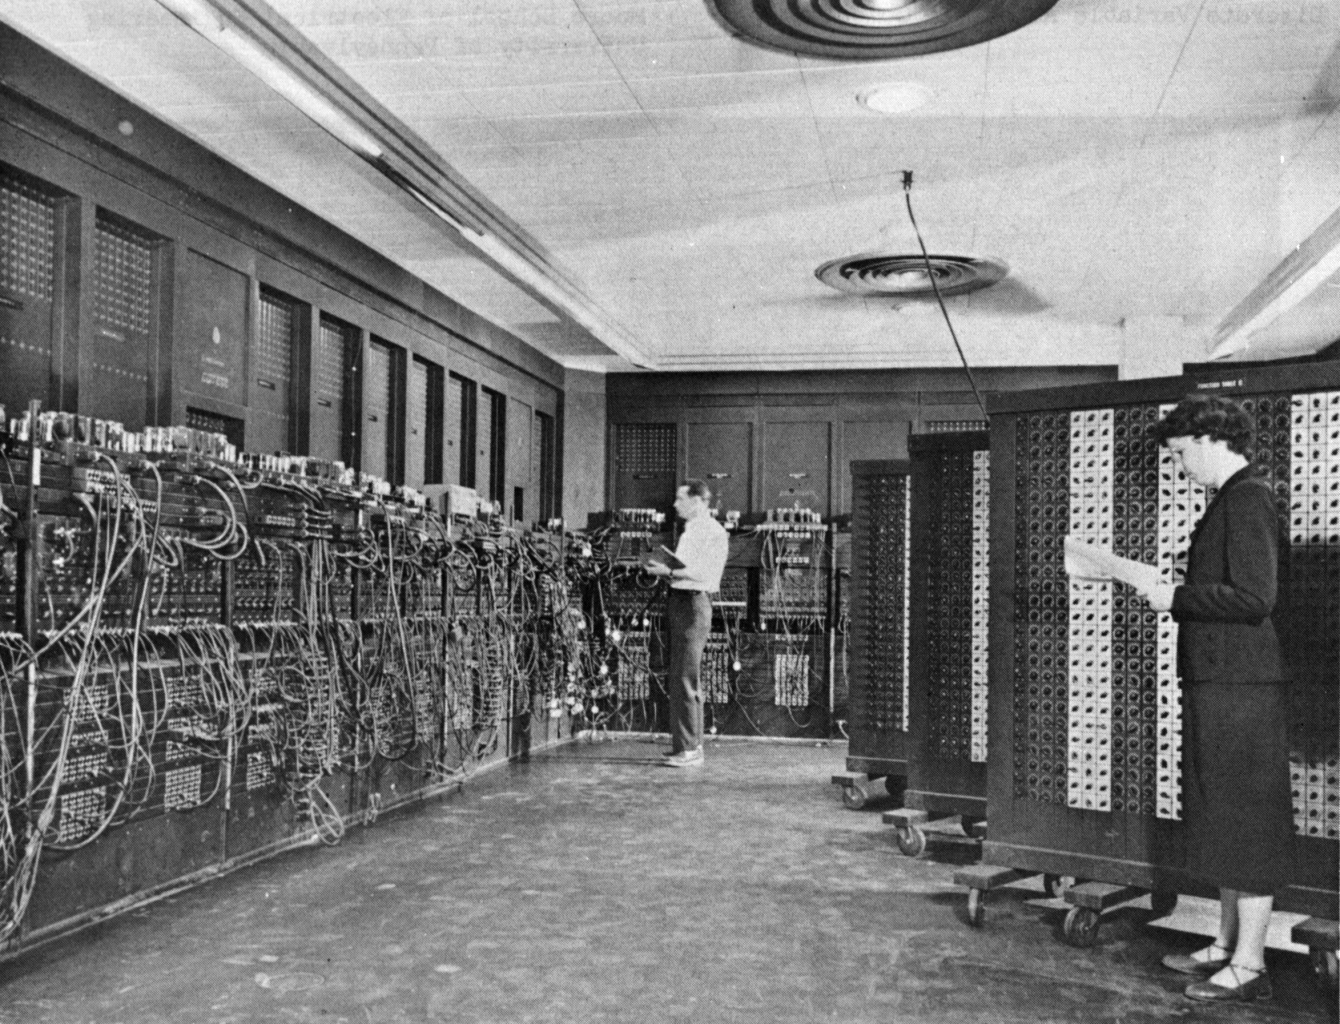
\includegraphics[width=4in]{Eniac}
  \end{center}
\end{frame}

\end{document}
